% !TEX root = main_vldb.tex
The definition of HD that we use is tailored for HL note, however, that it is the ones used in \cite{highway2013}. 
We now discuss how our results extend to the stronger definition.

The stronger version defines a path $P$ to be $r$-significant if, by adding at most one hop at each end, we get a shortest path $P'$ longer than $r$.
The path $P'$ is called an $r$-witness for $P$.
Intuitively, a path is significant if it represents a long path.
Observe that, if $P\in\PS$ is such that $\ell(P)>r$, then $P$ is $r$-significant by definition.
We remark also that a path can have many $r$-witnesses.

Finally, the path neighborhood must also be strengthened.
The path $P\in\PS$ belongs to $\Sf_r(v)$ if, $P$ has some $r$-witness $P'$ such that $\dist(v,P')\leq 2r$.
The reverse neighborhood $\Sb_r(v)$ is defined analogously.
With this modified versions of $r$-significant and neighborhood, the notions of LSHS and HD are the same as our previous definitions.

The benefits of this stronger notion are as follows.
If the HD is $h$, then $\Delta\leq h$ and $\alpha\leq h+1$.
Additionally, it allows proving results for CH, which the weaker definition cannot handle.
We finish by recalling that CHD and HD can be off by a factor of $n$.
The analogous for LSHS is still true even for this stronger notion.

\begin{proposition}\label{prop:treelike}
For any $h$, we can construct a family of networks such that the sparsity of LSHS is $h$ and that of EPHS is arbitrarily worse than $h$.
\end{proposition}
\begin{proof}
First, we construct an example where the sparsity grows from $h$ to $h^2$.
Consider an $h$-ary tree rooted at $u$ with three levels, i.e., with $1+h+h^2$ nodes.
Now add a node $v$ with $h$ children as in Figure~\ref{fig:treelike}. 
The grandchildren of $v$ are the same as the grandchildren of $u$.

All the edges are bidirectional and have unit cost.
The lengths are as follows: $ux_i$ and $vy_i$ (dashed in Figure~\ref{fig:treelike}) are zero; $uv$ and from $y_i$ to the leafs is one; from $x_i$ to the leafs is three.
It is easy to see that the sparsity of a LSHS is $h+1$.

On the other hand, every leaf $w$ is a $2$-efficient path.
Indeed, it can be extended to $x_iw$ that is the shortest path from $x_i$ to $w$ with constraint 1.
All the leafs are in the ball $B_4(u)$, so the sparsity is at least $h^2$.

\begin{figure}
\centering
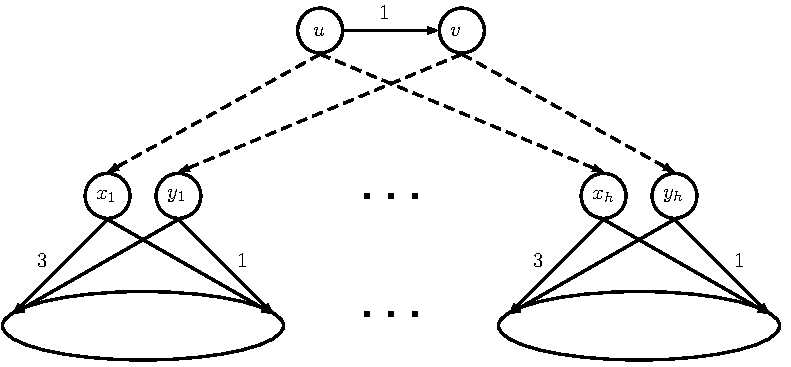
\includegraphics[scale=0.5]{TexImg/Treelike.pdf}
\caption{Example where CHD is much larger than the HD.}\label{fig:treelike}
\end{figure}

The general case works in the same fashion.
We make the sparsity grow to $h^k$ by creating two complete, $k$-level, $h$-ary trees $T$ and $T'$.
Connect the root of $T$ to the root of $T'$ and the leafs of both trees are shared.
Observe that the number of nodes is 
\begin{align*}
n &=[\text{$k$-level $h$-ary tree}] + [\text{$(k-1)$-level $h$-ary tree}]\\
&= ({h^{k+1}-1})/({h-1}) + ({h^k-1})/({h-1}),
\end{align*}
therefore the sparsity is $\Theta(n)$, the worst possible.
\end{proof}